\documentclass[10pt,professionalfonts,aspectratio=169]{beamer}

% usar pdflatex

% codificacion
\usepackage[utf8]{inputenc}
\usepackage[T1]{fontenc}
\usepackage[spanish,es-tabla,es-noshorthands]{babel}
\usepackage{csquotes}
\usepackage{booktabs}
\usepackage{amsmath}
\usepackage{amsfonts}
\usepackage{amssymb}
\usepackage{bm}
\usepackage{siunitx}
\usepackage{tikz}
\usepackage{graphicx}
\usepackage{grffile}

% colores
\definecolor{burgundy}{RGB}{128, 0, 32}
\definecolor{darkwine}{RGB}{90, 0, 20}
\definecolor{softwine}{RGB}{250, 240, 242}
\definecolor{charcoal}{RGB}{40, 40, 40}

\usetheme{Madrid}
\usecolortheme{default}

\setbeamercolor{palette primary}{bg=burgundy,fg=white}
\setbeamercolor{palette secondary}{bg=darkwine,fg=white}
\setbeamercolor{palette tertiary}{bg=black,fg=white}
\setbeamercolor{structure}{fg=burgundy}
\setbeamercolor{title}{fg=burgundy,bg=white}
\setbeamercolor{titlelike}{fg=burgundy}
\setbeamercolor{frametitle}{fg=white,bg=burgundy}
\setbeamercolor{author}{fg=charcoal}
\setbeamercolor{date}{fg=charcoal}

\setbeamercolor{block title}{bg=burgundy,fg=white}
\setbeamercolor{block body}{bg=softwine,fg=black}
\setbeamercolor{block title example}{bg=charcoal,fg=white}
\setbeamercolor{block body example}{bg=gray!10,fg=black}

\setbeamercolor{item}{fg=burgundy}
\setbeamercolor{subitem}{fg=darkwine}
\setbeamertemplate{sections/subsections in toc}[sections numbered]

\setbeamertemplate{navigation symbols}{}
\setbeamertemplate{caption}[numbered]
\setbeamertemplate{frametitle continuation}[from second]
\setbeamerfont{caption name}{series=\bfseries}

% bibliografia
\usepackage[
    backend=biber,
    style=apa,
    sortcites=true,
    sorting=nyt,
    language=auto
]{biblatex}
\addbibresource{references_slices.bib}

\hypersetup{
    colorlinks=true,
    citecolor=blue,
    linkcolor=white,
    urlcolor=blue
}

% graficos
\graphicspath{{../Plots/}{Plots/}}

% metadatos
\titlegraphic{\includegraphics[height=2.5cm]{"bonita (1).png"}}
\logo{%
  \ifnum\insertframenumber>1%
    \includegraphics[height=0.8cm]{"bonita (1).png"}%
  \fi%
}

\title[Tasas de Interés y Tipo de Cambio]{Tasas de Interés y Tipos de Cambio}
\subtitle{Desviaciones de la Paridad Descubierta en México y Colombia (2018--2023)}
\author[Grupo 4]{E.~López \and H.~Pérez \and K.~Pozo \and E.~Chavarría \and F.~Torrez}
\institute[UNI-DACIP]{Grupo 4 \\ Economía Internacional Real \\ Universidad Nacional de Ingeniería (UNI) --- DACIP}
\date[\,]{\today}

\begin{document}

% 1 portada
\begin{frame}[plain]
    \setbeamercolor{title}{fg=white,bg=burgundy}
    \setbeamercolor{subtitle}{fg=white}
    \titlepage
\end{frame}

% 2 introduccion
\begin{frame}{Introducción}
    \begin{block}{Punto de partida teórico}
        Según la Paridad Descubierta de Tasas de Interés (UIRP), las diferencias en tasas entre países deben compensarse con cambios esperados en el tipo de cambio. Si un banco central sube su tasa por encima de la de EE.~UU., su moneda debería depreciarse a futuro en una proporción equivalente \parencite{krugman2012}.
    \end{block}

    \begin{block}{Caso de estudio y pregunta de investigación}
        México y Colombia frente al dólar (2018--2023). Ambos con tipo de cambio flexible y metas de inflación, pero con estructuras productivas distintas. \\
         ¿En qué medida las desviaciones de la UIRP se explican por \textbf{primas de riesgo} en lugar de variaciones puras en las expectativas cambiarias?
    \end{block}
    
\end{frame}

% 3 hipotesis
\begin{frame}{Hipótesis}
    \begin{itemize}
        \item La UIRP \textbf{no se cumple de forma exacta} en la práctica.
        \item Las desviaciones fomentan el \textbf{carry trade} en México, impulsado por su alta liquidez cambiaria.
        \item En Colombia están condicionadas por los \textbf{términos de intercambio}, especialmente los precios del petróleo.
        \item La transmisión monetaria opera de forma distinta al modelo básico en cada economía.
    \end{itemize}
\end{frame}

% 4 marco teorico enfoque de activos
\begin{frame}{Marco Teórico: Enfoque de Activos}
    Las divisas se comportan como activos financieros cuyo precio presente depende de las expectativas sobre su valor futuro \parencite{krugman2012}.

    \begin{block}{Rentabilidad esperada en moneda nacional}
        \centering
        $(R^* + (E^e - E))/E$
    \end{block}

    \begin{itemize}
        \item $R^*$: tasa de interés externa (EE.~UU.).
        \item $E$: tipo de cambio nominal presente (pesos por dólar).
        \item $E^e$: tipo de cambio esperado para el periodo siguiente.
    \end{itemize}

    \vspace{0.2cm}
    Si se anticipa una depreciación futura ($E^e$ sube), la rentabilidad en dólares sube, los inversores demandan dólares hoy y $E$ sube hasta igualar rendimientos.
\end{frame}

% 5 marco teorico uirp
\begin{frame}{Paridad Descubierta de Tasas de Interés (UIRP)}
    \begin{block}{Condición de no arbitraje}
        \[
            \frac{R^* + (E^e - E)}{E} \;\longrightarrow\; R - R^* = \frac{E^e - E}{E}
        \]
    \end{block}

    \begin{itemize}
        \item $R$: tasa nacional (México o Colombia); \quad $R^*$: tasa externa (EE.~UU.).
        \item Si $R > R^*$, el peso debe depreciarse en el futuro en una proporción equivalente al diferencial.
        \item Si un banco central sube $R$ hoy, la UIRP predice una \textbf{apreciación inmediata} de la moneda local ($E$ baja) que genere la expectativa de depreciación compensatoria.
    \end{itemize}

    \vspace{0.1cm}
    \footnotesize\textit{Referencias:} \parencite{krugman2012,isard2006}
\end{frame}

% 6 marco teorico desviaciones
\begin{frame}{Desviaciones en la Práctica: Prima de Riesgo y Carry Trade}
    La UIRP falla a corto y mediano plazo: \textbf{forward premium puzzle}.

    \begin{block}{UIRP ampliada con prima de riesgo}
        \[
            R - R^* = \frac{E^e - E}{E} + \rho
        \]
    \end{block}

    \begin{itemize}
        \item $\rho > 0$: los inversores exigen rendimiento adicional por mantener activos locales.
        \item El \textbf{carry trade} (endeudarse en moneda de bajo interés e invertir en alto rendimiento) explota estas desviaciones, pero está expuesto a caídas abruptas cuando sube la aversión global al riesgo.
        \item \textcite{kalemli2021} muestran, con encuestas en 22 economías emergentes, que la prima UIP es \textbf{sistemáticamente positiva, más alta y volátil} que en economías avanzadas.
    \end{itemize}
\end{frame}

% 7 metodologia y datos
\begin{frame}{Metodología y Datos}
    \begin{block}{Fuentes}
        Series de tasas de interés de la OCDE vía FRED: EE.~UU., México y Colombia. Tipos de cambio MXN/USD (Reserva Federal) y COP/USD (OCDE), frecuencia mensual.
    \end{block}

    \begin{block}{Modelo de Fama \parencite{fama1984}}
        UIRP log-lineal:
        \[
            i_t - i_t^* = \mathbb{E}_t[\Delta s_{t+1}]
        \]
        Regresión de Fama:
        \[
            \Delta s_{t+1} = \alpha + \beta\,(i_t - i_t^*) + \varepsilon_{t+1}
        \]
        Hipótesis conjunta de insesgadez: $H_0: \alpha = 0$ y $\beta = 1$.
    \end{block}

    \footnotesize Estimación por MCO con errores estándar HAC Newey-West.
\end{frame}

% 8 resultados
\begin{frame}{Resultados de la Estimación}
    \begin{block}{México (MXN/USD)}
        \begin{itemize}
            \item $\hat{\beta} = 7{,}134$ \; (EE robusto $= 7{,}778$; $p = 0{,}363$) $\Rightarrow$ indistinguible de cero.
            \item $\hat{\alpha} = -27{,}619$ \; ($p = 0{,}283$).
            \item $R^2 = 1{,}18$\,\%; \; $\hat{\sigma} = 37{,}86$\,\%.
        \end{itemize}
    \end{block}

    \begin{block}{Colombia (COP/USD)}
        \begin{itemize}
            \item $\hat{\beta} = -2{,}830$ \; (EE $= 2{,}158$; $p = 0{,}195$) $\Rightarrow$ signo contrario (forward premium puzzle) pero no significativo.
            \item $R^2 = 2{,}53$\,\%; \; $\hat{\sigma} = 44{,}41$\,\%.
        \end{itemize}
    \end{block}

    \footnotesize En ambos casos el diferencial de tasas tiene poder predictivo nulo.
\end{frame}

% 9 caso mexico super peso
\begin{frame}{Caso México: El Súper Peso y el Carry Trade}
    \begin{block}{Paradoja 2018--2023}
        Banxico mantuvo tasas muy por encima de la Fed, pero el peso \textbf{se apreció} de forma sostenida en lugar de depreciarse como predice la UIRP.
    \end{block}

    \begin{itemize}
        \item \textbf{Carry trade:} crédito en dólares baratos $\to$ CETES con tasas $> 11$\,\% \parencite{banxico2024}.
        \item \textbf{Liquidez:} el MXN es la divisa emergente más negociada (24 h), con bajos costos de entrada/salida \parencite{imf2023}.
        \item \textbf{Relocalización (nearshoring):} flujos constantes de IED.
        \item \textbf{Remesas récord} y percepción de riesgo país controlada \parencite{benavides2016,imf2023}.
    \end{itemize}

    \vspace{0.2cm}
    \footnotesize Los flujos especulativos y la inversión real dominaron sobre las expectativas de depreciación del modelo.
\end{frame}

% 10 caso colombia uirp ampliada
\begin{frame}{Caso Colombia: UIRP Ampliada y Compresión Externa}
    Economía pequeña y abierta, dependiente de hidrocarburos y con presiones fiscales crecientes.

    \begin{block}{UIRP ampliada con prima de riesgo}
        \[
            i_t = i_t^* + \frac{E_t[S_{t+1}]}{S_t} + \rho_t
        \]
    \end{block}

    \begin{block}{Mecanismo 1: Compresión externa del diferencial}
        Cuando la Fed sube $i_t^*$, se reduce la liquidez internacional y el dólar se fortalece.
        \begin{itemize}
            \item 2022--2023: Fed en $5{,}25$--$5{,}50$\,\%.
            \item Banrep sube hasta $12$\,\% en diciembre de 2022.
            \item Los aumentos locales \textbf{apenas compensan} el endurecimiento global $\to$ menor atractivo relativo de los activos colombianos y presión sobre el peso.
        \end{itemize}
    \end{block}
\end{frame}

% 11 caso colombia prima de riesgo fisher
\begin{frame}{Caso Colombia: Prima de Riesgo y Tasa Real Negativa}
    \begin{block}{Mecanismo 2: Absorción por prima de riesgo y tasa real negativa}
        Según la ecuación exacta de Fisher:
        \[
            r_t = \frac{1 + i_t}{1 + \pi_t} - 1
        \]
        \begin{itemize}
            \item Inflación: $5{,}62$\,\% (2021) $\to$ $13{,}12$\,\% (2022).
            \item Tasa real: $-2{,}48$\,\% (2021) y $-0{,}99$\,\% (2022).
            \item Con riesgo país al alza, los activos en pesos pierden atractivo y el peso se deprecia.
        \end{itemize}
    \end{block}

    \begin{block}{Mecanismo 3: Ajuste endógeno de expectativas cambiarias}
        Caídas de términos de intercambio o déficits externos persistentes desplazan el TCR de equilibrio hacia niveles más depreciados, elevando $E_t[S_{t+1}]$ y anulando el arbitraje (Borradores de Economía Banrep 742, 901 y 1030).
    \end{block}
\end{frame}

% 12 caso colombia petroleo
\begin{frame}{Colombia: Dependencia Extrema del Petróleo}
    En 2023, petróleo y carbón = \textbf{52{,}3\,\%} de la balanza comercial; en 2022, el crudo concentró el \textbf{78{,}2\,\%} de las exportaciones a EE.~UU.

    \begin{block}{Tres canales de transmisión}
        \begin{itemize}
            \item \textbf{Comercial:} caída de exportaciones $\to$ menos divisas $\to$ mayor déficit de cuenta corriente y menor IED.
            \item \textbf{Financiero:} caída del crudo $\to$ mayor percepción de riesgo $\to$ crédito externo más caro $\to$ presión depreciatoria.
            \item \textbf{Fiscal:} menores ingresos petroleros afectan regalías, impuestos y dividendos de Ecopetrol $\to$ mayor déficit público.
        \end{itemize}
    \end{block}

    \footnotesize Estudios del Banrep confirman relación negativa entre precio del crudo y TRM.
\end{frame}

% 13 caso colombia evidencia
\begin{frame}{Colombia: Prima de Riesgo y Ruido Político (2018--2023)}
    \begin{itemize}
        \item \textbf{2020:} fuerte caída del crudo $\to$ depreciación del peso.
        \item \textbf{2022:} petróleo caro, pero el peso perdió valor por alzas de la Fed e incertidumbre económica.
        \item \textbf{2023:} petróleo bajó, pero el peso se apreció por mejores condiciones financieras y menor déficit externo.
    \end{itemize}

    \vspace{0.2cm}
    \begin{block}{Efectos distributivos}
        \begin{itemize}
            \item Peso fuerte $\to$ golpea a la industria nacional (importaciones más competitivas).
            \item Peso débil $\to$ ayuda a exportadores, pero encarece insumos y reduce poder de compra.
        \end{itemize}
    \end{block}

    \footnotesize El comportamiento del peso no depende solo del petróleo: también de factores monetarios, financieros y comerciales.
\end{frame}

% 14 conclusiones
\begin{frame}{Conclusiones}
    \begin{itemize}
        \item La UIRP \textbf{no se cumple} en México ni Colombia (2018--2023): el diferencial de tasas explica $< 3$\,\% de las variaciones cambiarias y los residuos presentan colas pesadas (se rompe la neutralidad al riesgo).
        \item En \textbf{México}, el diferencial de tasas impulsó el carry trade y apreció el peso: Súper Peso, alta liquidez, nearshoring \parencite{imf2023} y remesas.
        \item En \textbf{Colombia}, las alzas del Banrep fueron insuficientes por la dependencia del petróleo, el deterioro fiscal y el aumento de la prima de riesgo país.
        \item En ambas economías emergentes, el tipo de cambio estuvo dominado por \textbf{primas de riesgo y flujos de capital}, antes que por el diferencial de tasas.
    \end{itemize}
\end{frame}

% 15 anexo pruebas
\begin{frame}{Anexo: Pruebas de Estacionariedad y Normalidad}
    \begin{block}{Estacionariedad}
        ADF rechaza raíz unitaria al 5\,\%: México ($p = 0{,}020$), Colombia ($p = 0{,}010$). KPSS no rechaza estacionariedad ($p > 0{,}10$). Series $I(0)$.
    \end{block}

    \begin{block}{Normalidad de residuos}
        Shapiro-Wilk y Jarque-Bera rechazan normalidad ($p < 0{,}001$). Distribución leptocúrtica (colas pesadas, p.~ej.\ COVID), lo que contradice el supuesto de neutralidad al riesgo de la UIRP.
    \end{block}
\end{frame}

% 16 anexo graficos
\begin{frame}{Anexo: Análisis Gráfico}
    \begin{columns}[T]
        \begin{column}{0.32\textwidth}
            \centering
            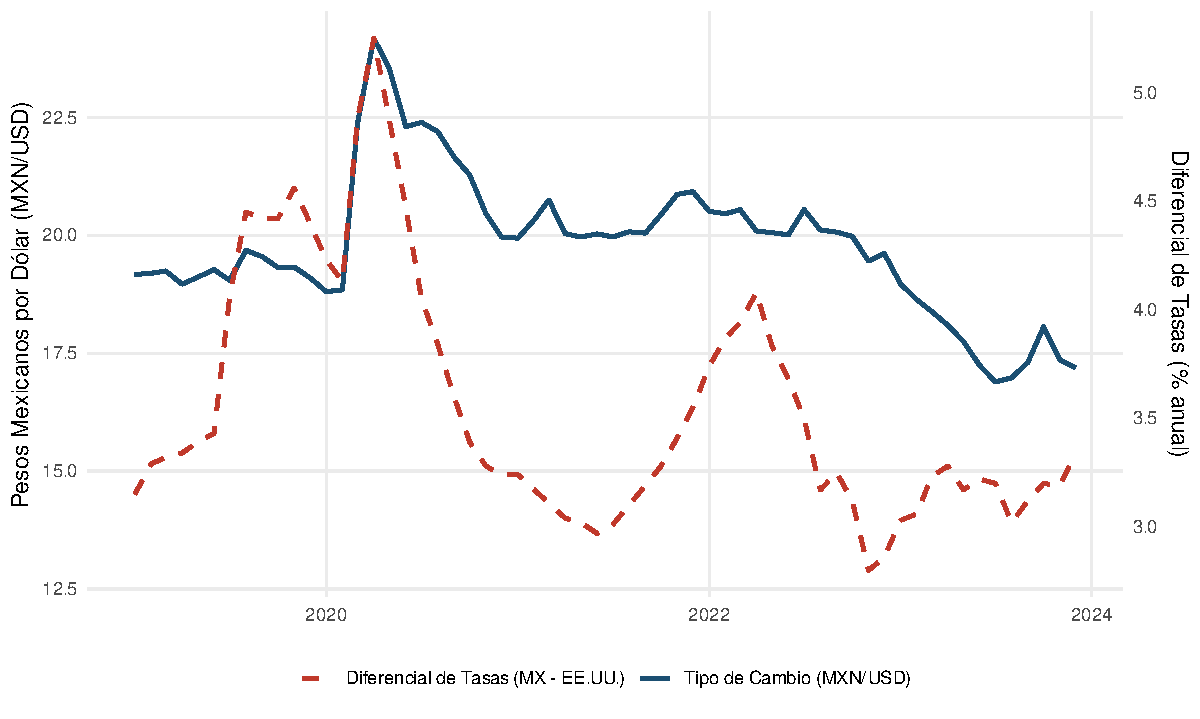
\includegraphics[width=\textwidth]{Figura1_Mexico_UIP.pdf}
            \par\vspace{0.1cm}\footnotesize México: tipo de cambio y diferencial
        \end{column}
        \begin{column}{0.32\textwidth}
            \centering
            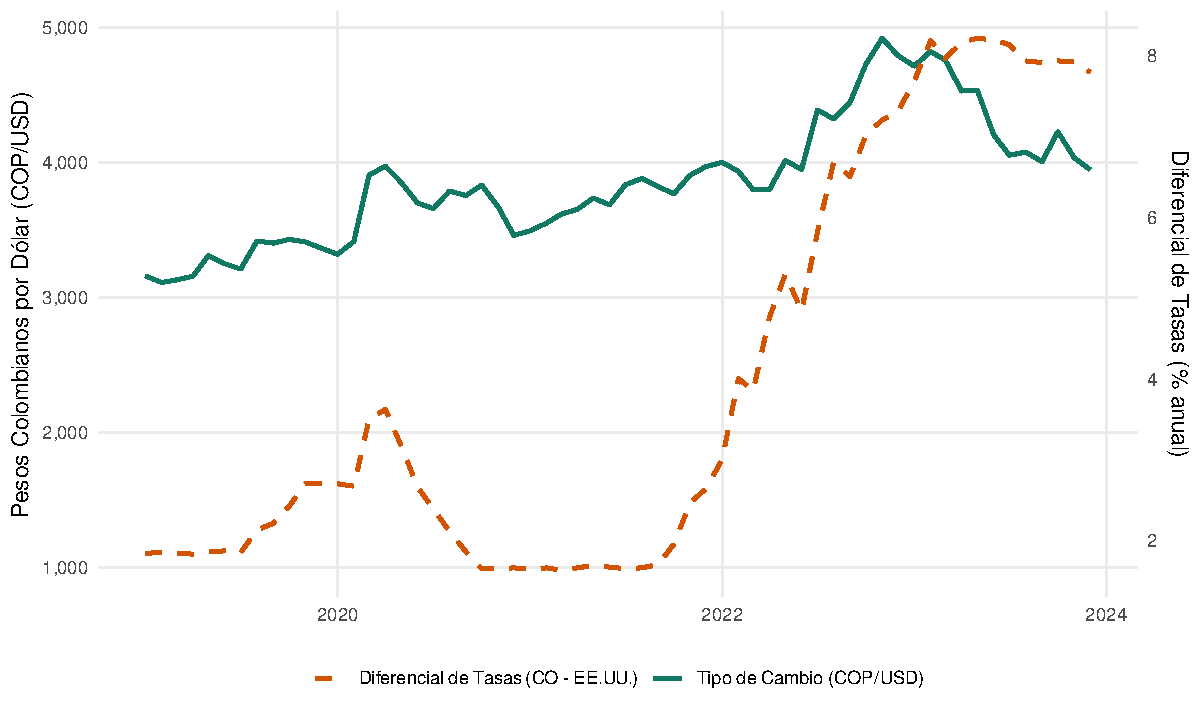
\includegraphics[width=\textwidth]{Figura2_Colombia_UIP.pdf}
            \par\vspace{0.1cm}\footnotesize Colombia: tipo de cambio y diferencial
        \end{column}
        \begin{column}{0.32\textwidth}
            \centering
            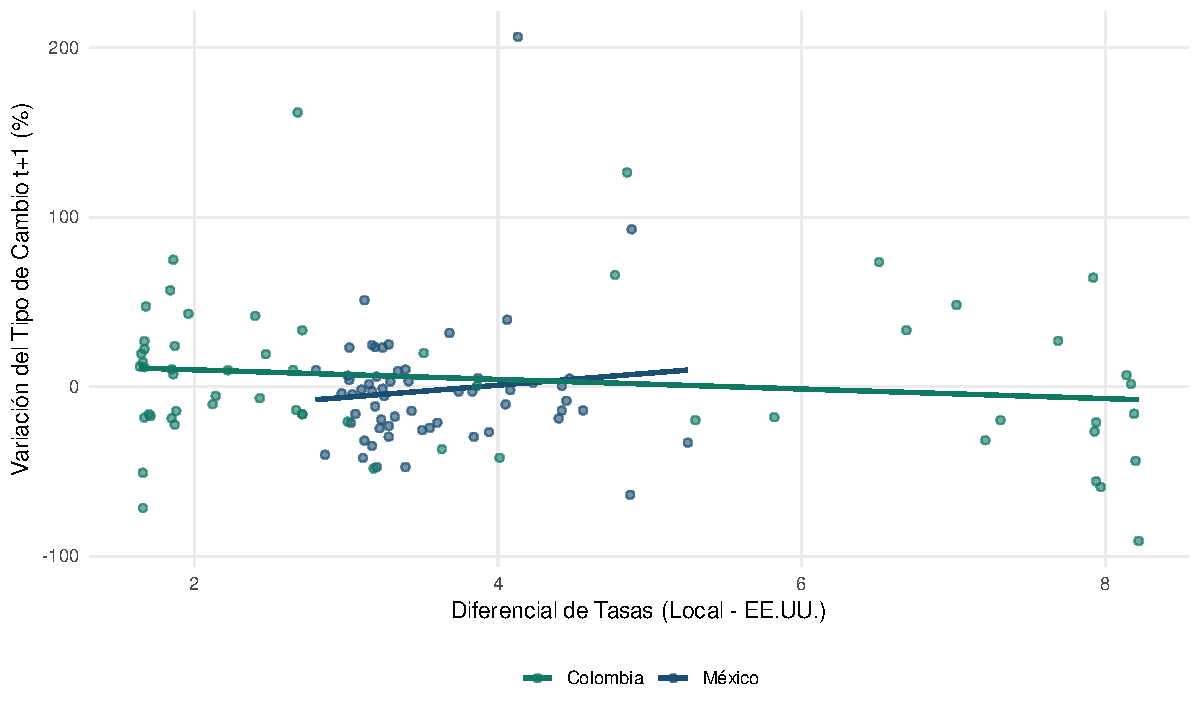
\includegraphics[width=\textwidth]{Figura3_regresion_UIP.pdf}
            \par\vspace{0.1cm}\footnotesize Dispersión y ajuste de Fama
        \end{column}
    \end{columns}

    \vspace{0.3cm}
    \footnotesize En ambos países los puntos se alejan de la línea teórica: bajo poder explicativo del modelo ($R^2 < 3$\,\%), colapso sistemático de la UIRP.
\end{frame}

% 17 referencias
\begin{frame}[allowframebreaks]{Referencias}
    \renewcommand*{\bibfont}{\scriptsize}
    \printbibliography[heading=none]
\end{frame}

% 18 cierre
\begin{frame}[plain]
    \centering
    \vspace{2cm}
    {\Huge \textbf{¡Muchas Gracias!}}\\[1cm]
    {\large ¿Preguntas o comentarios?}
\end{frame}

\end{document}